\documentclass[ wastespaceontitle, english]{cheat_sheet_template}
%\usepackage[english]{babel}
\usepackage{lipsum}

\usepackage{longtable}
\usepackage{xtab}
\usepackage{mathtools}

\veranstaltung{Chemistry}
\numberCols{3}

\newcommand{\tikzmark}[3]{\tikz[overlay,remember picture] \node  [anchor = north, xshift=#2,yshift=-1pt, text width=2cm, align=center] (#1){#3};}

\usetikzlibrary{positioning}
\usetikzlibrary{calc}

\begin{document}
% \subsubsection{common ions}
\subsubsection{Solubility Guidelines for Common Ionic Compounds in $H_2O$}
\begin{tabular}{p{0.3\linewidth}|p{0.6\linewidth}}
    Soluble, Ionic Compounds containing & Important Exceptions \\ \hline
     $NO_3^-$ & None\\
     $CH_3COO^-$ & None\\
     $Cl^-$ & Compounds of $Ag^+$ , $Hg_2^{2+}$ , and $Pb^{2+}$ \\
     $Br^-$ & Compounds of $Ag^+$ , $Hg_2^{2+}$ , and $Pb^{2+}$\\
     $I^-$& Compounds of $Ag^+$ , $Hg_2^{2+}$ , and $Pb^{2+}$\\
     $SO_4^{2-}$ & Compounds of $Sr^{2+}$ $Ag^+$ , $Hg_2^{2+}$ , and $Pb^{2+}$ \\ \hline
     Insoluble, Ionic Compounds containing & Important Exceptions \\ \hline
$S^{2-}$ & Compounds of $NH_4^+$ , the alkali metal cations,$ Ca^{2+}$ , $Sr^{2+}$ , and$ Ba^{2+}$ \\
$CO_3^{2-}$ & Compounds of $NH_4^+$ and the alkali metal cations\\
$PO_4^{3-}$ & Compounds of $NH_4^+$ and the alkali metal cations\\
$OH-$ & Compounds of $NH_4^+$ , the alkali metal cations, $Ca^{2+}$ , $Sr^{2+}$ , and$ Ba^{2+}$ \\
\end{tabular}   \\


% \subsubsection{types of reaction}
% combustion, decomposition


\section{Gases}
    \subsection{Ideal gas law}
    ideal gas: no intermolecular interactions between particles
    
    STP: 273.15 K, 1 atm = 101.325 kPa
    
    \eqbox{P V = n R T = N k_B T}
    \eqbox{\rho = \frac{P}{R T} M}
    Partial pressure \eqbox{P_i = \frac{n_i}{n_{tot}} P_{tot}}
    
    \begin{minipage}{0.69\linewidth}
    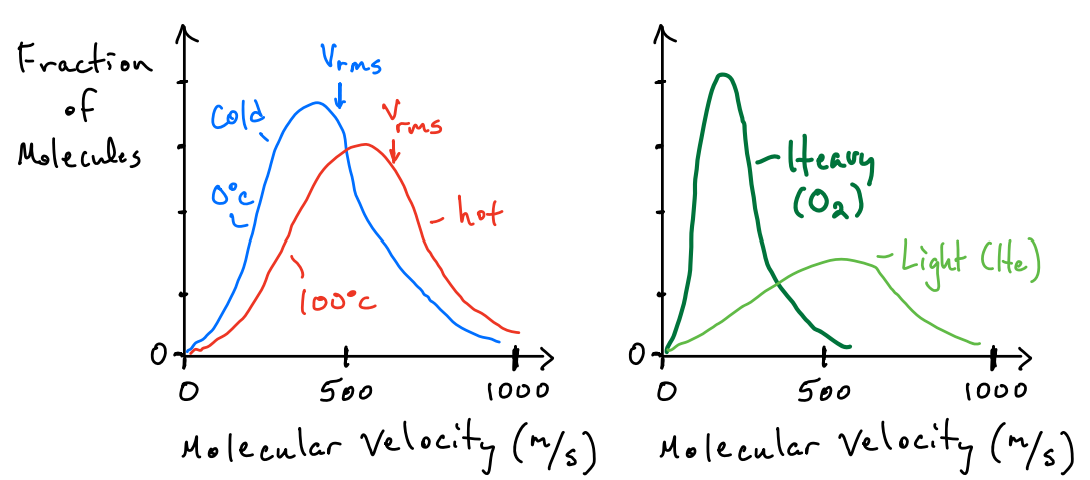
\includegraphics[width=1\linewidth]{pictures/Distrubution_velocity.png}
    \end{minipage}
    \begin{minipage}{0.3\linewidth}
        $v_{rms} = \sqrt{\frac{3 R T}{M}}$ 
        
        v molecules that have average kinetic energy (mean root squared velocity)
        
    \end{minipage}
    
    \subsubsection{Pressure measurement}
    \begin{minipage}{0.45\linewidth}
        Barometer $P = \rho g h$\\
        \begin{tikzpicture}
            \node[anchor=south west,inner sep=0] (image) at (0,0) {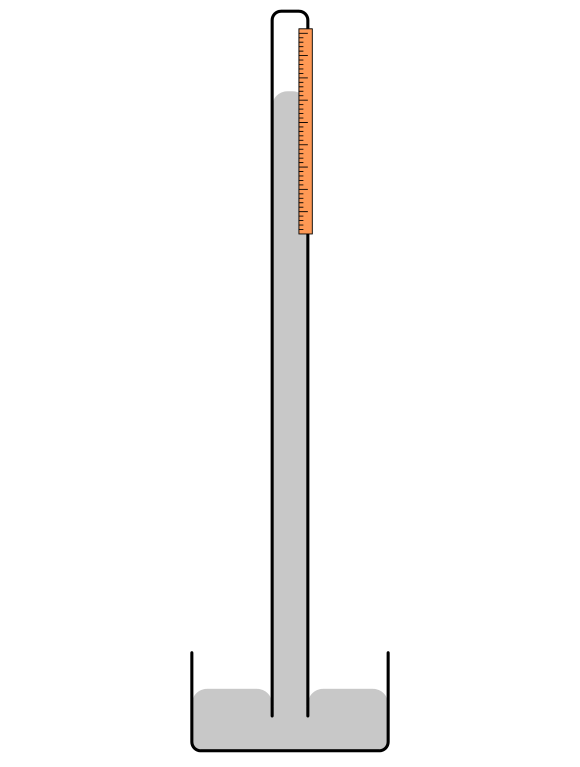
\includegraphics[width = 0.4\linewidth]{pictures/MercuryBarometer.png}};
             \begin{scope}[x={(image.south east)},y={(image.north west)}]
                \draw[<->,thick] (0.4,0.85) -- (0.4,0.1) node [pos = 0.5, left] {h};
                 \draw[->,thick] (0.6,0.4) -- (0.6,0.1) node [pos = 0.1, right] {P};
            \end{scope}
        \end{tikzpicture}
        
    \end{minipage}
    \begin{minipage}{0.45\linewidth}
        Manometer  $P_{gas} = P_{atm} + \rho g h$
        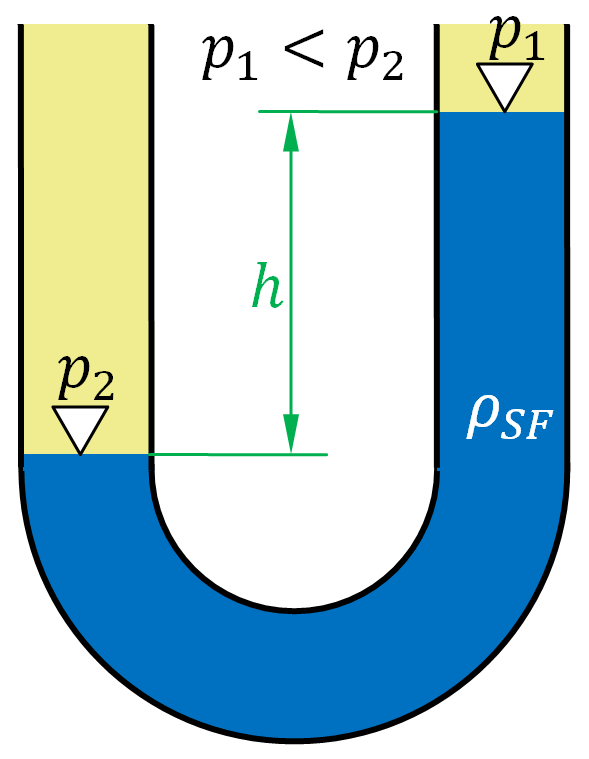
\includegraphics[width = 0.4\linewidth]{pictures/U-Rohr.png}
    \end{minipage}
    
    $P_{atm}= 101.325 kPa = 760mm Hg = 760 torr$ 
\section{Thermodynamics}
    \subsection{Ethalpy H}
        \eqbox{H = E + PV} 
        $ \Delta H  \stackrel{\dot{P}=0}{=}  q_p $
        \begin{itemize}
            \item $\Delta H > 0 \Rightarrow$ system gained heat
            \item $\Delta H < 0 \Rightarrow$ system lost heat
        \end{itemize}
        \text{state function: only depends on current state(p,V...)/path independent: E, H}
        \subsubsection{Hess's Law}
            \eqbox{\Delta H_{rxn} = \sum_i \Delta H_i} 
            \eqbox{\Delta H_{rxn}^0 = \sum_{prod, j} b_j \cdot \Delta H_{f,j}^0
            - \sum_{react,i} a_i \Delta H_{f,i}^0} \\
        \subsubsection{Bond enthalpy}
            \eqbox{\Delta H_{rxn} = \sum_{i : \text{bonds broken}} \Delta H_i - \sum_{i : \text{bonds formed}} \Delta H_i}  \\
        \subsubsection{Reactions}
            \begin{itemize}
                \item Spontaneous p. = p. occur w/o assistance
                \item Reversible = p. can be reversed w/no change to surroundings $infinitisimal$ change
                \item Irreversible = surroundings changed when process is reversed
            \end{itemize}
            \itembox{\begin{itemize} 
                \item All real p. are irreversible
                \item All spontaneous p. are real
                \item All spontaneous p. are Irreversible
                \item To return system to initial state $\Rightarrow$ requires work
                \item While E is conserved during spontaneous p. E tends to spread out and 
                become less usefull
            \end{itemize}}
        \subsubsection{3rd law of thermodynamics}
            \begin{itemize}
                \item Pure, crystalline solid substance at $T=0K$ has $S=0$
                \item For rxn: $\Delta S_{surr} = \frac{-q_{sys}}{T} = \frac{- \Delta H_{rxn}^0}{T}$ 
                \item $S = ln(W)*k_B$ whereas W increases with V,p,N, complexity of molecule
                \item Reversible p. : $\Delta S_{univ} =0$ and $\Delta G = 0$
                \item Irreversible p. : $\Delta S_{univ} > 0$ and $\Delta G > 0$
                \item Entropy of the universe increases for any spontaneous p
            \end{itemize}
    \subsection{Gibb's free energy}
    \text{maximum amount of work can extract from}
        \begin{itemize}
            \item \eqbox{G := H - T S}
            \item at const. T $ \Rightarrow \Delta G= \Delta H_{sys} - T \Delta S_{sys}$
        \end{itemize}
        \begin{tabular*}{\linewidth}{l l l l l}
            $\Delta H$ & $\Delta S$ & $- T \Delta S$ & $\Delta G$ & Rxn Characties \\
            \hline
            - & + & - & - & \\
            + & - & + & + & \\
            - & - & + & + or - & \\
            + & + & - & + or - & 
        \end{tabular*}

     \subsection{Thermodynamics of solution}
     calorimetry: \eqbox{\Delta H_{rxn} = q_{rxn} = -q_{H_2O}} \\
     \eqbox{\Delta Q = c_s*m* \Delta T = c_m *n * \Delta T} 
     1 cal = 4.182 J
     
     solvent + solute $\xrightleftharpoons[disolve]{crystallize}$ solution
     \begin{align}
        (solvent)_n &\to n \cdot solvent &\Delta H_{solvent} (separate solvent) \\
        (solute)_m &\to m \cdot solute &\Delta H_{solute} (separate solute) \\
        n \cdot solvent +  m \cdot solute   &\to solution &\Delta H_{mix} ( mix separate solvent \& solute) \\ \hline
         (solvent)_n + (solute)_m &\to solution &\Delta H_{soln} (total enthalpy change) \notag
     \end{align}
     \begin{itemize}
         \item $\Delta H_{soln} > 0 \Rightarrow - T \Delta S_{soln}$ musst be sufficient $\Rightarrow$ more likely at high T 
         \item $\Delta H_{soln} < 0$ typically forms solution for any $c(solute)$, completly miscible (mixable)
     \end{itemize}
     \subsubsection{Lattice energy and phase diagram}
     \begin{minipage}{0.45\linewidth}
         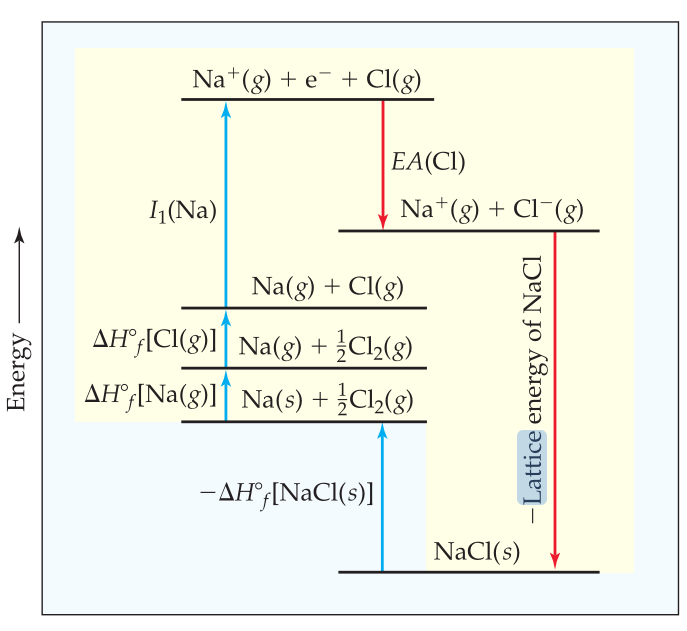
\includegraphics[width=1 \linewidth]{pictures/lattice_energy.png}
     \end{minipage} 
     \begin{minipage}{0.45\linewidth}
         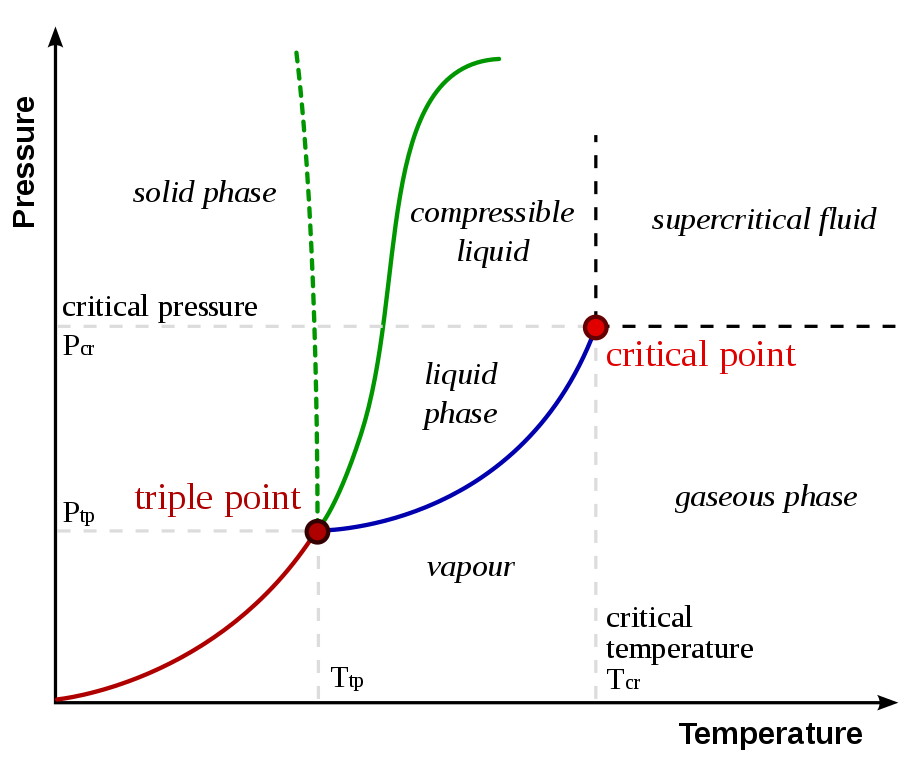
\includegraphics[width=1 \linewidth]{pictures/phasediagram.png}
     \end{minipage}
     \text{supercritical fluid: no distinction between liquid and gas, no surface tension}
     \subsection{Factors affecting solubility}
     \begin{itemize}
         \item strong solute-solvent interactions favor higher solubility
         \item substances with similar interactions tend to be soluble in each other
         \item \textbf{Temperature}
         \begin{itemize}
             \item Ion solubility in $H_2O$ increases with T $\Rightarrow \Delta S_{soln} > 0$
             \item Gas solubility in $H_2O$ decreases with T $\Rightarrow \Delta S_{soln} < 0$
         \end{itemize}
         \item \textbf{Pressure} \eqbox{S_g = k P_g} $S_g$ gas solubility, $k$ Henry's law constant, $P_g$ partial pressure 
     \end{itemize}
     \subsubsection{ Colligative Properties}
     = Solute effects liquid, depends only on amount of solute
     
     \text{ideal solution: solvent-solvent and solute-solvent interaction are the same}
     \begin{itemize}
         \item Boiling point elevation \eqbox{\Delta T_{bp} = T_{bp}^{soln} -T_{bp}^{soln} = i K_b m }, m = molarity of solute, $K_b$ = molal bp elevation constant, 
         i = van't Hoff factor = $\begin{cases}
             1,\text{ for non-electrolytes} \\
             \#\text{ ions produced, for electrolytes}
         \end{cases}$
         \item Vapor - pressure lowering Raoult's law: \eqbox{P_{vap}^{soln} = X_{solvent} \cdot P_{vap}^{pure}}
         \item Freezing - point depression \eqbox{\Delta T_{fp} = - i K_{f} m}
         \item Osmotic pressure \eqbox{\Pi = i M R T } $\Pi$ osmotic pressure to counteract osmotic flow
         \item hypertonic $\Pi > \Pi_{ref}$ and hypotonic $\Pi < \Pi_{ref}$
     \end{itemize}
     \subsubsection{Expressions of concentration}
     \begin{tabular}{cccc}
         x & mole fraction $= \frac{n(\text{solute})}{n_{tot}}$ &  & mass\% = $ \frac{m(\text{solute})}{m_{tot}}$ \\
         c & molarity $= \frac{n(\text{solute})}{V_{tot}}$ & $M$ & ppm = mass\% $\cdot 10^6$ \\
         b & molality $= \frac{n(\text{solute})}{m(\text{solvent})}$ & $m = \frac{mol}{kg}$ & ppb = mass\% $\cdot 10^9$ 
     \end{tabular}
     \subsection{Properties of liquids}
    \begin{itemize}
       \item  viscosity: resitsance to flow, interactions slow flow
       \item surface tension: Energy unit per area of liquid surface, minimize surface where intermol. interactions are missing
        \item vapor pressure: pressure of molecules  in gas phase (volatile liquid has small $E_{int}$ and high $p_v$
    \end{itemize}
    
    \subsubsection{Clausius-Clapeyron equation}
   $\ln P_{vap} = - \frac{\Delta H_{vap}}{R T} + C$ 
   

\section{Chemical Kinetics}
    \eqbox{\text{Reaction rate: } |\dot{c} (A)|}
    For general rxn: $\alpha A + \beta B \to \gamma C + \delta D$
     $\textbf{Rate}=- \frac{1}{\alpha} \frac{d [A]}{dt}= - \frac{1}{\beta} \frac{d [B]}{dt} = \frac{1}{\gamma} \frac{d [C]}{dt} = \frac{1}{\delta} \frac{d [D]}{dt}$ \\
    \subsection{Rate laws}
    \begin{itemize}
        \item general \eqbox{\text{Rate } = k [A]^n [B]^m \cdots}
        \item m,n reaction orders
        \item $m,n \in \{0, \frac{1}{2}, 1,2, \cdots\}$
        \item m,n are \underline{not} necessarily equal $\alpha, \beta$
        \item overall reaction order $= m + n + \cdots$
        \item fast rxns $k > 10^9$ slow rxns $k < 10$
    \end{itemize}
    \subsubsection{Using rate laws rxn $A \to B$}
    \begin{itemize}
        \item$ - \frac{d[A]}{dt} = k [A]^m$
        \item First-order $m = 1$: \eqbox{\ln [A]_t - \ln[A]_0 = - k t}  \eqbox{t_{1/2} =  \frac{\ln{2}}{k}}
        \item Second-order $m=2$ :  \eqbox{\frac{1}{[A]_t} = k t + \frac{1}{[A]_0}} \eqbox{t_{1/2} =  \frac{1}{k [A]_0}}
        \item Zero-order $m=0$:    \eqbox{[A]_t = - k t + [A]_0} \eqbox{t_{1/2} =  \frac{[A]_0}{2 k}}
    \end{itemize}
    \subsection{Collision model}
    \subsubsection{Temperature dependence of rate law}
    \begin{itemize}
        \item $k(t) = (\text{collision per time}) \cdot (\text{fraction of collisions properly oriented}) \cdot  (\text{fraction molecules with } E > E_A) $ %the larger E_A the slower the reaction
        \item \eqbox{k(t) = A \cdot \exp{\frac{-E_A}{R T}}} 
        \item $ln(\frac{k_1}{k_2})= \frac{E_A}{R} (\frac{1}{T_2} -\frac{1}{T_1} )$ for typical $E_A, T$, rxn rate doubles for $\delta T = + 10K$ 
    \end{itemize}
    \subsubsection{Elementary reactions}
    \begin{itemize}
        \item simple step where 1 'thing' happens, typically 1 bond breaks/forms
        \item \fcolorbox{black}{white}{\vspace{2pt} $m=\alpha$ and $n=\beta$ for elementary rxn \vspace{2pt}}
        \item process to determine rxn mechanism \begin{enumerate}
            \item measure rates
            \item propose mechanism
            \item check consistency
        \end{enumerate}
    \end{itemize}
    \subsection{Law of mass action}
    
    \eqbox{K = \frac{k_{forward}}{k_{reverse}} = \frac{(a_C)^\gamma (a_D)^\delta}{(a_A)^\alpha (a_B)^\beta }} \eqbox{a_i = \begin{cases}
        \frac{[i]}{1 M} \\
        \frac{P_i}{1 \textbf{bar}}
    \end{cases}}\eqbox{K_P  = K_C (R T)^{\Delta n}}  
    \begin{itemize}
        \item note: requires closed system
        \item all rxns are elementary near equilibrium
        \item $K$ is rxn specific
        \item $K_C$ \& $K_P$ are unitless
        \item for pure solids/liquids $a = 1$ 
        \item for multistep rxn $K = \Pi_i K_i$
        \item rate-limiting step: k1 $<<$ k2 $\rightarrow$ rate overall is only dependent on k1 
    \end{itemize}
    Reaction quotient \eqbox{Q = \frac{[C]^\gamma [D]^\delta}{[A]^\alpha [B]^\beta }}
    \begin{itemize}
        \item $Q < K$ forward rxn forms more product
        \item $Q > K$ reverse rxn forms more reactant
    \end{itemize}
    \itembox{Le Chatelier Principle: If a system at equil. is disturbed by change in $T,P$ or $c$ system shifts its equil. to counteract disturbance}\\
    
    endothermic: $A + \Delta E \rightleftharpoons B$ and exothermic: $A \rightleftharpoons \Delta E + B$
    
    V decreases $\rightarrow$ p increases $\rightarrow$ reaction is preferred which produces less molecules
    
    Relation to thermodynamics:
    \eqbox{\Delta G = \Delta G^0 + R T \ln Q }  
    
    At equil.: $\Delta G = 0 \Rightarrow \Delta G^0 = - R T \ln K$  
 
     
    \section{Electronic Structure}
        \begin{itemize}
            \item $c = \lambda * f$
            
            \item Rydberg Equ: $ E_H = \frac{h c}{\lambda_H} = h c R_H (\frac{1}{n_1^2} - \frac{1}{n_2^2})$
            \item Orbitals 
            \begin{itemize}
                \item principal quantum number, $n \in \{1, ...\}$
                \item angular quantum number, $l \in \{1 ... , n-1\}$ \begin{tabular}{c|c|c|c}
                        0 & 1 & 2  & 3  \\ \hline
                         s & p & d & f
                    \end{tabular}
                \item Magnetic quantum number, $m_l \in \{ -l, ... ,l\}$ (orientation in space)
                \item Spin magnetic quantum number, $m_s \in \{-\frac{1}{2}, \frac{1}{2}\}$
                \item Ex. Se: $[Ar]3d^{10}4s^24p^4$
            \end{itemize}
        \end{itemize}
        \subsubsection{Pauli exclusion principle}
        \begin{itemize}
            \item Order of subshells ? $\to$ use periodic table $s=2, p=6, d =10, f=14$
            \item Hunds rule
            \item Exception: half/filled orbitals are more favourable
        \end{itemize}
        \subsubsection{Screening}
        \begin{itemize}
            \item For given shell(s) v.e. repelled by core e ('screen') $\Rightarrow$ v.e. feel $Z_{eff} < Z$ 
            Effect stronger for subshells further from nucleus 
            \item Trends
        \end{itemize}
        \begin{center}
            \begin{tikzpicture}
            \node[anchor=south west,inner sep=0] (image) at (0,0) {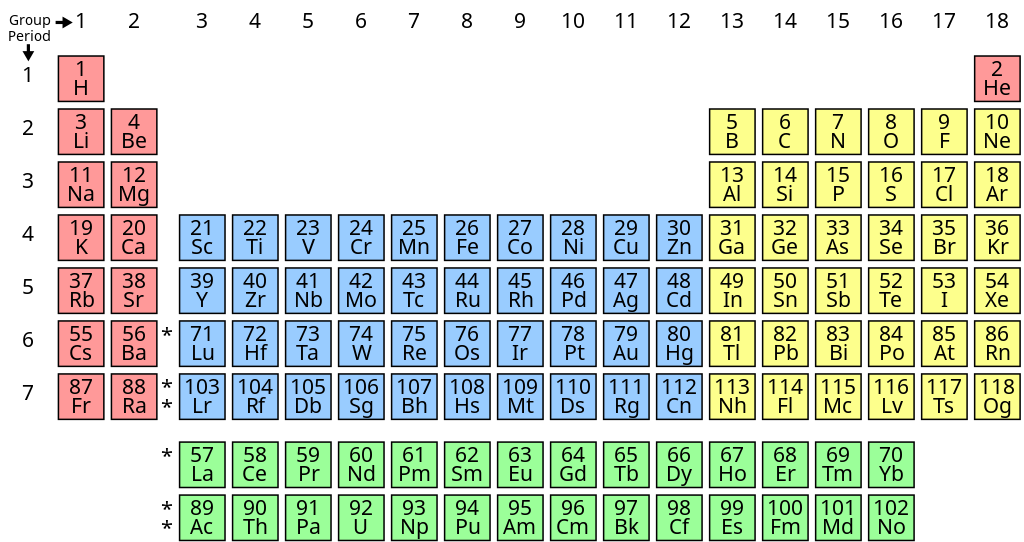
\includegraphics[width=0.9\linewidth]{pictures/Periodic_Table.png}};
             \begin{scope}[x={(image.south east)},y={(image.north west)}]
                \draw[->,thick] (0.1,.2) -- (.8,.9);
                \draw[->,thick] (0.8,.8) -- (0.05,0.05) node [pos=0.5,below right,draw, fill = white] {increasing atomic radius};
                \node[draw,align=left, fill = white] at (0.3,0.7) {increasing electro \\ negativity \\ionization energy \\affinity};
            \end{scope}
        \end{tikzpicture}
        \end{center}
    \subsection{Bonds}
    \subsubsection{Bond polarity}
    \begin{itemize}
        \item If electro negativity $\geq 2 \Rightarrow$ ionic bond 
    \end{itemize}
    \subsubsection{Dipol Moments}
    \begin{itemize}
        \item $ |\Vec{\mu}| = Q r$ 
        \item pointing from - to +
        \item very polar bonds $\Rightarrow$ large $ |\Vec{\mu}|$
    \end{itemize}
    \subsubsection{Ionic vs covalent}
    \begin{itemize}
        \item continuum of behavior 
        \item more covalent $\Rightarrow$ 'molecular behavior' low melting/boiling T
        \item more ionic $\Rightarrow$ ionic solid brittle high boiling T
        \item electro negativity difference not perfect: oxidation \# of metals increases  $\Rightarrow$  bonding more covalent 
    \end{itemize}
    
    \subsection{Molecular geometry}
    \text{domain: bonding + nonbonding pairs} 
    
    \text{molecular geometry: just position of atoms}

    \subsubsection{Drawing Lewis Structures}
    \begin{itemize}
        \item Octet rule Atoms want 8 v.e.'s
    \end{itemize}
    \begin{enumerate}
        \item sum v.e.'s of all atoms
        \item write symbols and connect with single bonds
        \item complete octets around non-central atoms
        \item place remaining v.e.'s around central atom
        \item try multiple bonds if central atom doesn't have octet
    \end{enumerate}
    \subsubsection{Exceptions to the octet rule}
    \begin{itemize}
        \item odd \# e 
        \item less then octet v.e.'s
        \item more then octet of v.e.'s
    \end{itemize}
    \subsubsection{Formel charge}
    \begin{itemize}
        \item  Formel Charge = 
        v.e.'s - $\frac{1}{2}$ atom's bonding e's - atom's non-bonding e's
        \item dominent Lewis structure have formel charges closet to 0, and $\ominus$ on more electro negative atoms
    \end{itemize}
    \subsubsection{Valance-shell electron pair repulsion}
    \begin{enumerate}
        \item draw Lewis
        \item count e domains
        \item determine e domain geometry
        \item determine molecular geometry from position of atoms
    \end{enumerate}
                

\setlength\tabcolsep{2pt}
\begin{longtable}{lllll}
    \hline
    \#& electron domain geometry & molecular geometry & angle & examples \\
    \hline
            2& 
            \centering
                 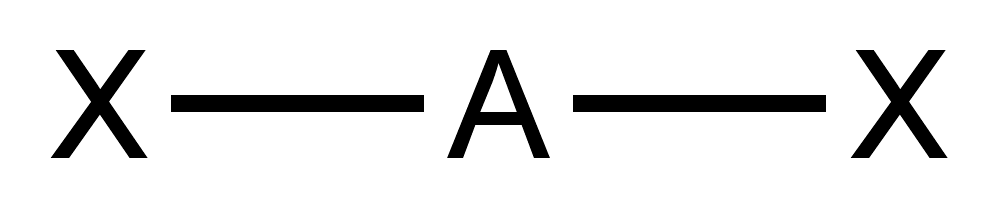
\includegraphics[width = 0.2\linewidth]{edomaingeo/AX2E0-2D.png} 
                 $AX_2$
                  & linear & $180^\circ$ & $H_2$ \\
            \hline
            3&  \centering
                 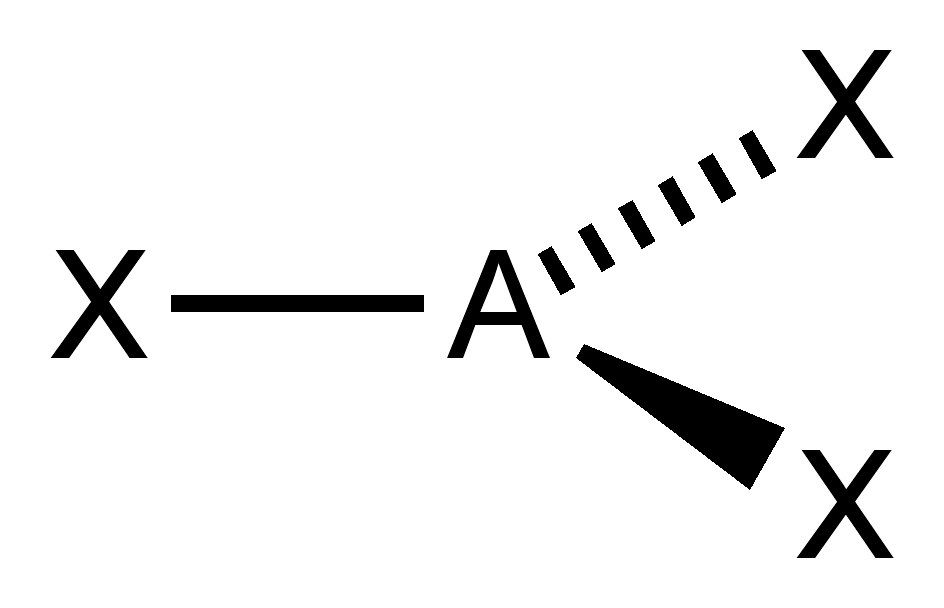
\includegraphics[width = 0.2\linewidth]{edomaingeo/AX3E0-side-2D.png} 
                 $AX_3$
                  & triangular planar & $120^\circ$ & $NO_3^-$ \\
            &  \centering
                 % \includegraphics[width = 0.2\linewidth]{edomaingeo/AX2E1-2D.png} 
                 $AX_2E_1$
                  & bent & $\approx 115^\circ$ & $SO_2$ \\
         
            \hline
            4&  \centering
                 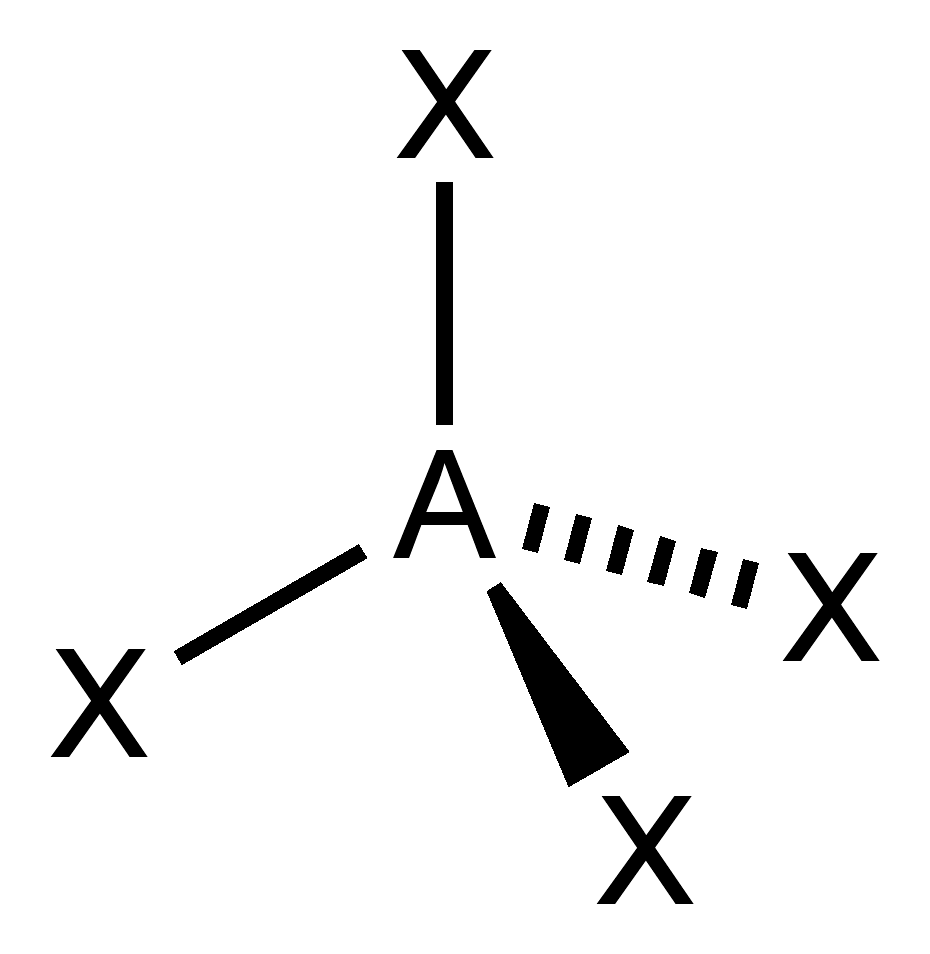
\includegraphics[width = 0.2\linewidth]{edomaingeo/AX4E0-2D.png} 
                 $AX_4$
                  & tetrahedral &  $109.5^\circ$ & $CH_4$ \\
            &  \centering
                 % \includegraphics[width = 0.2\linewidth]{edomaingeo/AX3E1-2D.png} 
                 $AX_3E_1$
                  & trigonal planar & $\approx 107^\circ$ & $NH_3$ \\
            &  \centering
                 % \includegraphics[width = 0.2\linewidth]{edomaingeo/AX2E2-2D.png} 
                 $AX_2E_2$
                  & bent & $\approx 104^\circ$ & $H_2O$  \\
             \hline
            5&  \centering
                 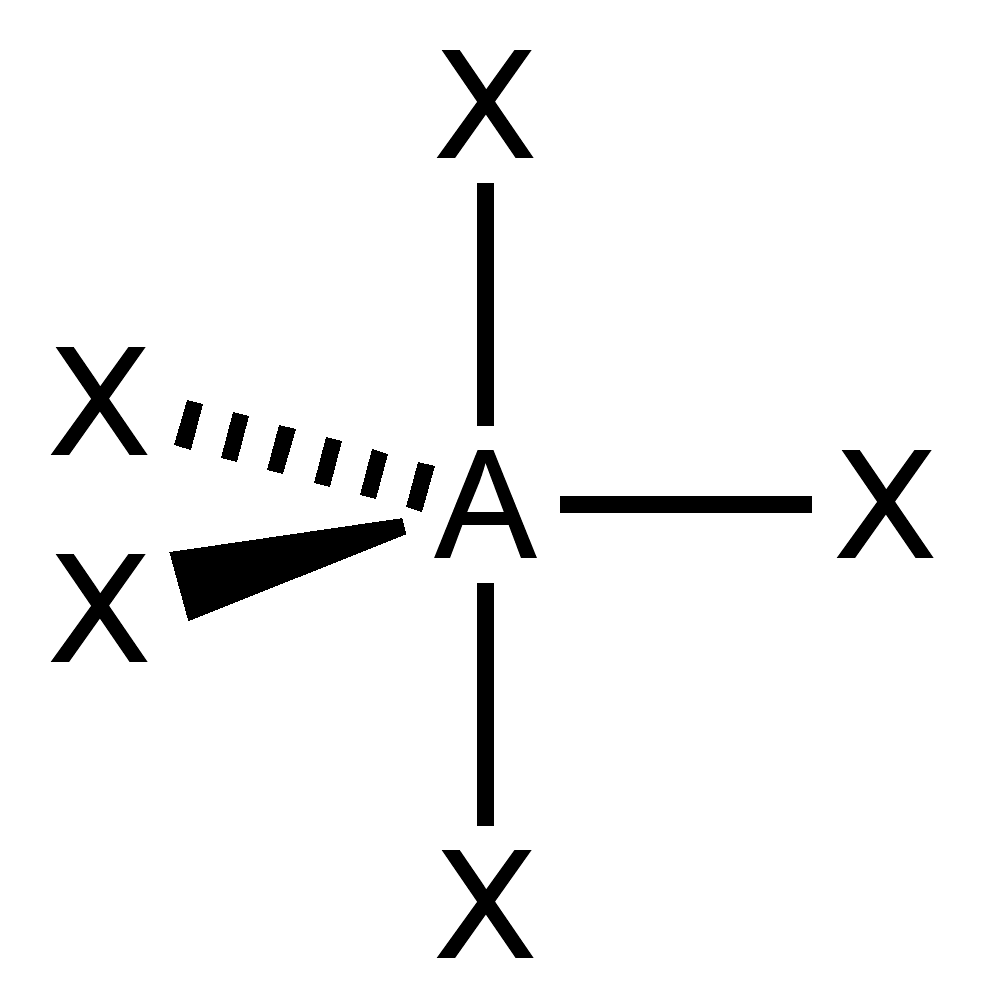
\includegraphics[width = 0.2\linewidth]{edomaingeo/AX5E0-2D.png} 
                 $AX_5$
                  & trigonal bipyramidal & $90^\circ/ 120^\circ$& $PCl_5$ \\
            &  \centering
                 % \includegraphics[width = 0.2\linewidth]{edomaingeo/AX4E1-2D.png} 
                 $AX_4E_1$
                  & seesaw & $\approx 175^\circ/ 110^\circ$ & $SF_4$  \\
       
            &  \centering
                 % \includegraphics[width = 0.2\linewidth]{edomaingeo/AX3E2-2D.png} 
                 $AX_3E_2$
                  &  T-shape &  $\approx 87.5^\circ$ & $ClF_3$ \\
            &  \centering
                % \includegraphics[width = 0.2\linewidth]{edomaingeo/AX2E3-2D.png} 
                $AX_2E_3$
                & linear &  & $XeF_2$  \\
                \hline
            6&  \centering
                 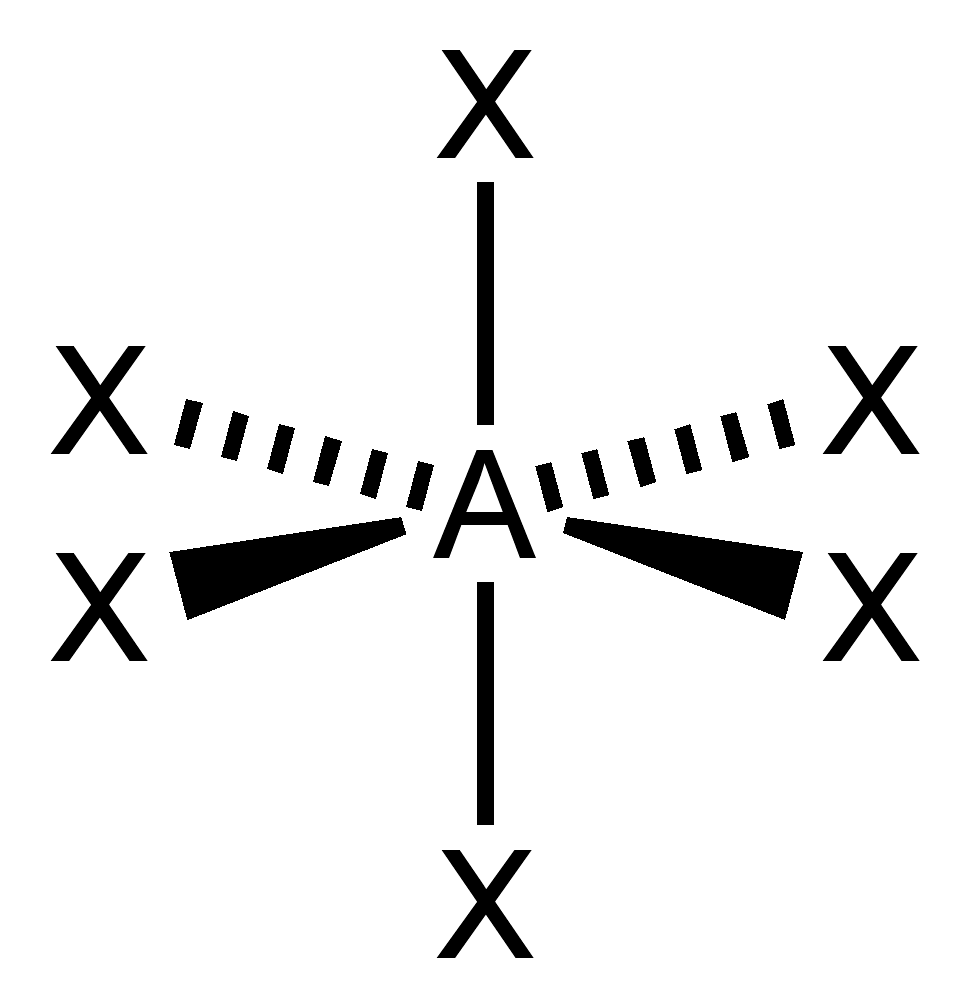
\includegraphics[width = 0.2\linewidth]{edomaingeo/AX6E0-2D.png} 
                 $AX_6$
                  & octahedral &  $90^\circ$ & $SF_6$ \\
            &  \centering
                 % \includegraphics[width = 0.2\linewidth]{edomaingeo/AX5E1-2D.png} 
                 $AX_5E_1$
                  & square pyramidal &  $\approx 85^\circ$ & $BrF_5$  \\
            &  \centering
                 % \includegraphics[width = 0.2\linewidth]{edomaingeo/AX4E2-2D.png} 
                 $AX_4E_2$
                  & square planar &  $90^\circ$ &  $XeF_4$ \\
                \hline
            7&  \centering
                 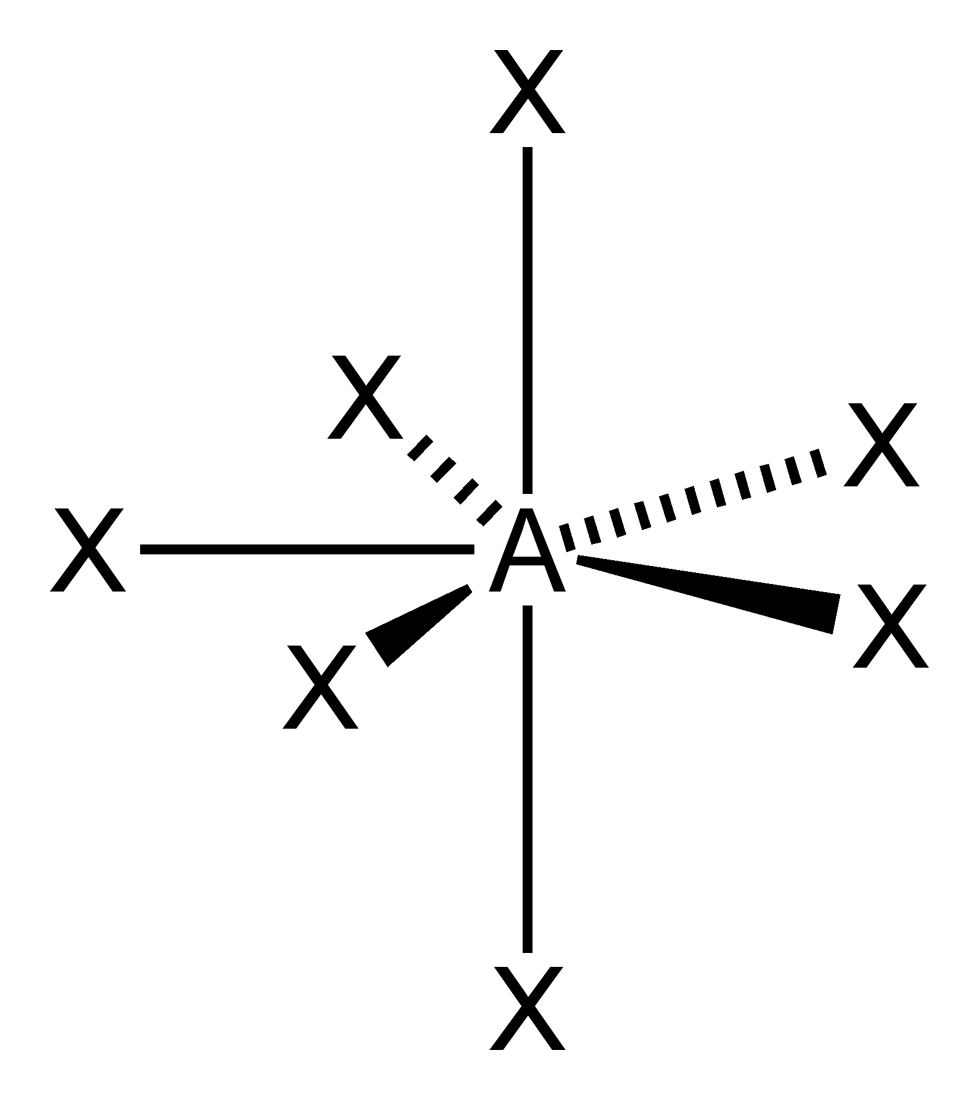
\includegraphics[width = 0.2\linewidth]{edomaingeo/AX7E0-2D.png} 
                 $AX_7$
                  & pentagonal bipyramidal  & $90^\circ/ 72^\circ$ & $IF_7$\\
           
            &  \centering
                 % \includegraphics[width = 0.2\linewidth]{edomaingeo/AX6E1-2D.png} 
                 $AX_6E_1$
                  & pentagonal pyramidal & $\approx 90^\circ/ \approx 72^\circ$ &  $XeOF_5^-$  \\
            &  \centering
                 % \includegraphics[width = 0.2\linewidth]{edomaingeo/AX5E2-2D.png} 
                 $AX_5E_2$
                  & pentagonal planar & $72^\circ$ & $XeF_5^-$  \\
                  \hline
\end{longtable} 

    \subsection{Intermolecular forces}
    
    \begin{tabular}{c c c}
        ion-dipole & $>$ H-bonding & $>$ dipole-dipole \\ & & $\approx$ dispersion \\
         $>50 kJ/mol$ & $\approx 25  kJ/mol$  & $\approx 10 kJ/mol$
         
    \end{tabular} \\
    
    Only for charged molecules: ion-ion \& ion-dipol interaction
    
    For neutral molecules:\\
    \subsubsection{A Dispersion}
    Induced dipole attractive at short distance \\
    \subsubsection{B Dipole-dipole polar molecules}
    Molecular dipoles interact $\Rightarrow$ attractive $E_{int}$ over short distance\\
    \subsubsection{A + B = van der Waals forces}
    \begin{itemize}
        \item always present
        \item increase with molecular size
        \item effected by shape
    \end{itemize}
    \subsubsection{Hydrogen bonding}
    \begin{itemize}
        \item in molecules with $N-H, O-H, F-H$
        \item $N,O,F$ very electro negative, small $\Rightarrow$ very polar
        %\item $H^{\delta_+}$ attracted to unbonded $e^-$'s on N,O,F small so H 
    \end{itemize}
    




\section{Acid Base}
    \subsubsection{Auto-ionization of water}
    \begin{itemize}
        \item $2 H_2O \rightleftharpoons OH^-(aq) + H_3O^+(aq)$
        \item $K_C = [OH^-] \cdot [H_3O^+] \equiv K_W = \text{ ion-product const } = 1.0 \cdot 10^{-14} (25^\circ C)$
    \end{itemize}
    \subsubsection{Acid-base pairs}
    \begin{itemize}
        
        \item generic rxn of acid with $H_2O$:   \\
         \( \tikzmark{B}{0.25cm}{base}H_2O + \tikzmark{AH}{0.2cm}{acid} AH \; \to \; \tikzmark{BH}{0.25cm}{conjugate\\acid} H_3O^+ \enspace + \enspace \tikzmark{A}{0.25cm}{conjugate\\base}A^- 
        \tikz[overlay,remember picture] \draw[<->] let \p1 = (B.south), \p2 = (BH.south), \n1 = {min(\y1,\y2) - 0.2cm } in  (\x1, \y1 ) --  (\x1, \n1 ) --  (\x2, \n1 ) -- (\x2, \y2);
        \tikz[overlay,remember picture] \draw[<->] let \p1 = (A.south), \p2 = (AH.south), \n1 = {min(\y1,\y2) - 0.25cm } in  (\x1, \y1 ) --  (\x1, \n1 ) --  (\x2, \n1 ) -- (\x2, \y2);
        \vspace{0.6cm} 
    \) \qquad $K_A = \frac{[A^-][H_3O^+]}{[HA]}$ \\
    
     \item generic rxn of base with $H_2O$:   
     
         \( \tikzmark{B}{0.25cm}{acid}H_2O + \tikzmark{AH}{0.1cm}{base} B \; \to \; \tikzmark{BH}{0.25cm}{conjugate\\base} OH^- \enspace + \enspace \tikzmark{A}{0.25cm}{conjugate\\acid}HB^+ 
        \tikz[overlay,remember picture] \draw[<->] let \p1 = (B.south), \p2 = (BH.south), \n1 = {min(\y1,\y2) - 0.2cm } in  (\x1, \y1 ) --  (\x1, \n1 ) --  (\x2, \n1 ) -- (\x2, \y2);
        \tikz[overlay,remember picture] \draw[<->] let \p1 = (A.south), \p2 = (AH.south), \n1 = {min(\y1,\y2) - 0.25cm } in  (\x1, \y1 ) --  (\x1, \n1 ) --  (\x2, \n1 ) -- (\x2, \y2);
        \vspace{0.8cm} 
    \)\qquad $K_B = \frac{[HB^+][OH^-]}{[B]}$
    \item amphiprotic substance: can act as both acid \& base, ex:  $H_2O, HCO_3^-, \cdots$
    \item each acid/base has its conjugate base/acid
    \end{itemize}
    
  
    
    \subsubsection{Strength of acids and bases}
      \begin{minipage}{0.5\linewidth}
     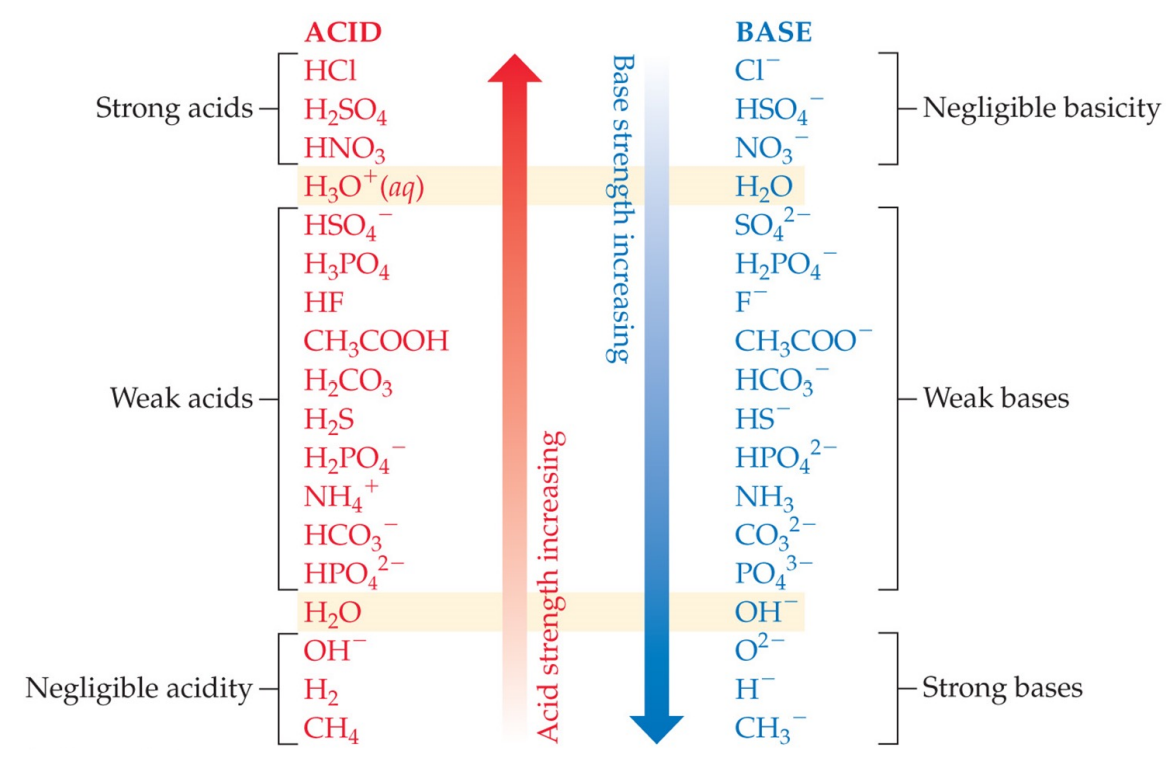
\includegraphics[width = \linewidth]{pictures/Strong acid base.png}
    \end{minipage}
    \begin{minipage}{0.49\linewidth}
     \begin{itemize}
        \item \eqbox{\text{pH} = - \log [H^+]} 
        \eqbox{\text{pOH} = - \log [OH^-]}
        \item \eqbox{pK_W  = 14.00  = \textbf{pH} + \textbf{pOH}}
        \item the smaller $pK_A = - \log K_A$/ $pK_B$ , the stronger acid/base
    \end{itemize}
    \end{minipage}
    
    \subsubsection{Common-ion effect}
    Add common ion to manipulate acid-base equil. \\Ex:
    \(CH_3COOH + H_2O \rightleftharpoons CH_3COO^- + H_3O^+\)
    Add strong electrolyte: $CH_3COONa\rightarrow$ Shifts acid-base equil left, decreasing $[H_3O^+]$\\
    \subsubsection{Buffer}
    \begin{itemize}
        \item weak acid-base conjugate pair $HA/A^- \Rightarrow$ protect against $H^+/OH^-$
        $HA + OH^- \rightleftharpoons A^- + H2O$ \quad
        $[H_3O^+] = K_A \frac{[HA]}{[A^-]}$\\
        $A^- + H_3O^+ \rightleftharpoons HA + H2O$ 
        \item as long as disturbance $\ll [A^-] \land [HA] \Rightarrow \Delta \textbf{pH} \approx 0$
        \item \text{Henderson–Hasselbalch equation, only useful for } 
        
        \eqbox{\textbf{pH} = pK_A + \log \frac{[\textbf{base}]}{[\textbf{acid}]}} $ [\textbf{acid}], [\textbf{base}]$ concentration of weak acid/conjugate base, for $K_A \ll [\textbf{acid}], [\textbf{base}]$
    \end{itemize}

    \section{Electrochemistry}
    \subsection{Redox equations}
    \subsubsection{Acidic aqueous solution}
    \begin{enumerate}
        \item divide into oxidation \& reduction
        \item balance \begin{itemize}
            \item balance elements not H/O
            \item balance O by adding $H_2O$
            \item balance H by adding $H^+$
            \item balance charge by adding $e^-$
        \end{itemize}
        \item multiply each half rxn to equate $e^-$
        \item add half rxn
        \item check
    \end{enumerate}
    \subsubsection{Basic aqueous solution}
    \begin{enumerate}
        \item balance half rxns as if in acidic solution
        \item add $\#H^+$ of $OH^-$ to each side 
        \item multiply each half rxn to equate $e^-$
        \item add half rxns
        \item check
    \end{enumerate}
    \subsection{Batteries}
    \begin{minipage}{0.35\linewidth}
          \begin{itemize}
        \item rxns $\Delta G < 0 \Rightarrow$ can extract electric work
        \item anode - oxidation
        \item cathode - reduction
    \end{itemize}
    
    \end{minipage}
     \begin{minipage}{0.55\linewidth}
     Galvanic cell:\\
     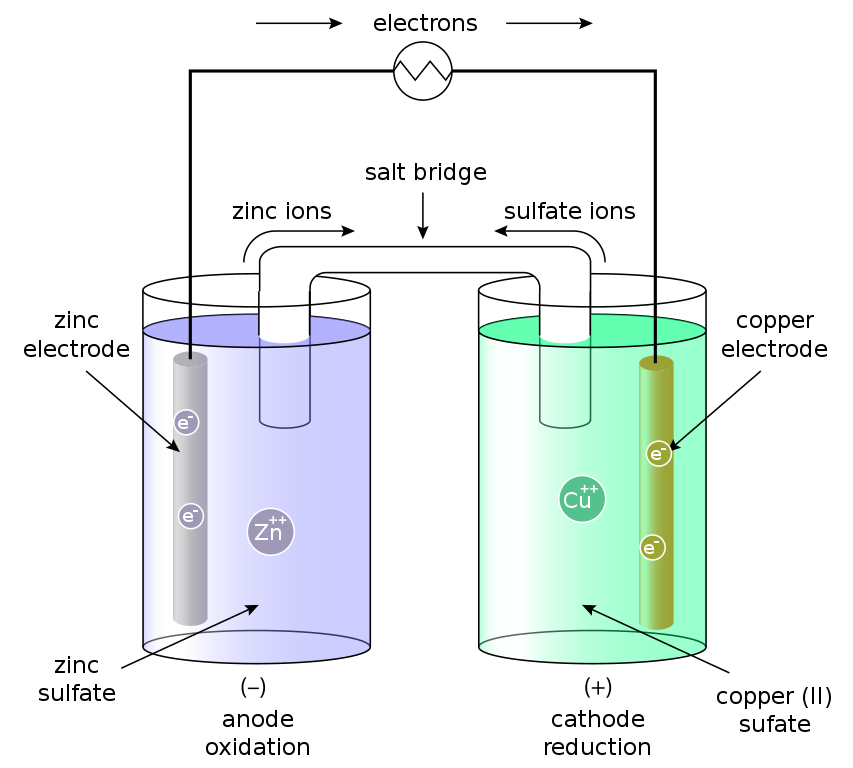
\includegraphics[width = \linewidth]{pictures/Galvanic_cell.png}
    \end{minipage}

    \subsubsection{Energy \& batteries}
    \begin{itemize}
        \item $E_{cell}^0 =$ cell voltage at standard conditions $(298.15K,1 \textbf{atm})$
        \item standard reduction potential $e \cdot E^0_{red} =$ pot. energy available if reduced
        \item \eqbox{E_{cell}^0 =E_{red}^0 - E_{ox}^0 = E_{cathode}^0-E_{anode}^0}
        \item to be useful/spontaneous reaction $E_{cell}^0 >0$
        \item at anode lower potential
        \item $E_{cell}^0$ is intensive
        \item $E_{red}^0$ half cell can't measured directly $\Rightarrow$ standard hydrogen electrode
        \item \eqbox{\Delta G = - n F E^0_{cell}}
    \end{itemize}

\subsection{Disclaimer}
No guarantee of correctness

\end{document}